\chapter{Solution Idea} \label{chap:solutionideas}

This section presents our plan for obtaining the objectives discussed in section \ref{chap:intro}. 
In our approach, we propose a Model-based and Data-driven development approach using the LEAN development process. 
As mentioned earlier, LEAN contains three phases Build, Measure, and Learn.
In the \texttt{Build} phase, we plan to create the \texttt{(1) Visualization of Prototypes}, and \texttt{(2) Model} these prototypes for Experiments and Tasks.
In the \texttt{Measure} phase, we plan to \texttt{(3) Assign these prototypes to the users} and measure the \texttt{(4) Experiment and the Task measurements}.
Finally, in the \texttt{Learn} phase, we would analyze the results performing \texttt{(5) Different analyses}, and \texttt{(6) Improve our Prototype} from the analyses feedback.  

Consider an example of a \textbf{``A video streaming service''} called \texttt{VideoStreamer (VS)}.
We divide the different stakeholders of this company into developers (e.g., programmers, designers, etc.) and non-developers (e.g., product owners).
% \begin{figure}
%     \centering
%     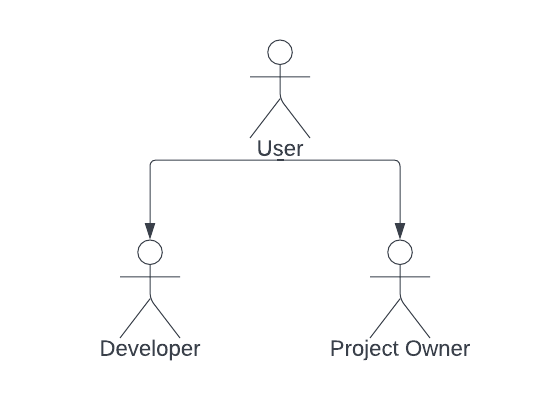
\includegraphics[scale=0.2]{images/solution-ideas/Stakeholder.png}
%     \caption{Different Stakeholders in the Company VS}
%     \label{solutionideas:fig:stakeholders}
%\end{figure}
Usually, the developers are responsible for developing various features required for the company. 
But, the problem is, in the beginning, knowing which design fits better for a UI is impossible. 
Therefore, we need to perform experiments on the UI using A/B testing.
So, the developers develop different variants for experimenting with the UI and get feedback from the non-developers.
This feedback process wastes a lot of time, so our solution is to give freedom to the product owners and reduce the gap between the product owners and the developers by allowing the product owners to create the UI using UI prototyping.

\section{Build}
In this step (as per figure \ref{intro:fig:lean}), we create ideas for the product and visualize the Prototypes (explained in section \ref{solutionideas:subsection:visualize}) and then Model them together for creating Experiments and Tasks for the users (explained in section \ref{solutionideas:subsection:modelling}).
We plan to implement the build step in a low-code or no-code technique for our solution because it needs negligible installation, setup, training, and implementation work.
The low-code or no-code technique enables software applications' rapid creation and deployment with little or no coding effort.

\subsection{Visualising the Prototypes}
\label{solutionideas:subsection:visualize}

We plan to create a system for non-developers to modify the UI elements in a canvas-like structure in an application using UI Prototyping.
For this, the non-developers first create a canvas screen and input the name for that screen.
As shown in figure \ref{solutionideas:fig:uiprototyping}, they can add UI elements like buttons, input buttons, select buttons, etc., on the canvas screen.
We propose to use angular\footnote{Angular: \url{https://angular.io/}} for developing the application.
Various UI elements are available for the drag and drop of the UI elements, as shown in figure \ref{solutionideas:fig:uiprototyping} (right side).

\begin{figure}[h]
    \centering
    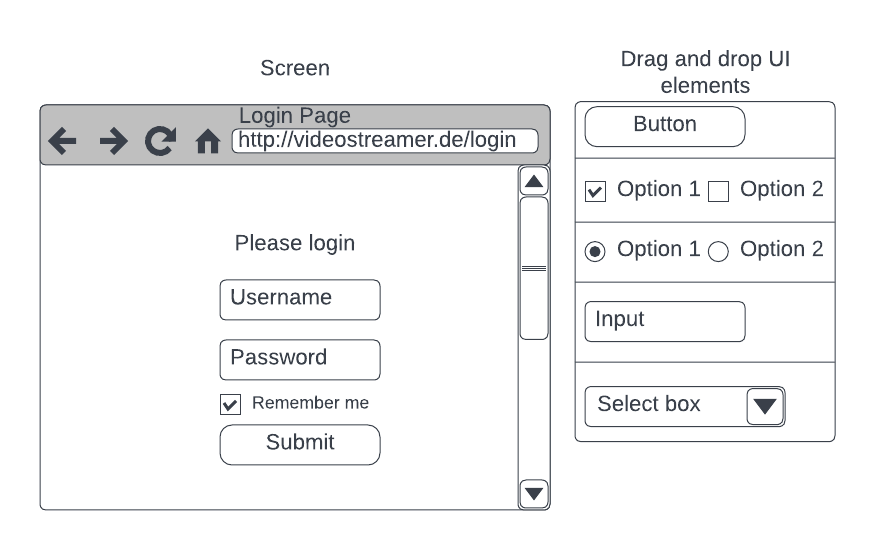
\includegraphics[scale=0.4]{images/solution-ideas/UIPrototyping.png}
    \caption{UI Prototyping using drag and drop of UI elements}
    \label{solutionideas:fig:uiprototyping}
\end{figure}

Once the non-developers finalize the UI screen, they can move to the next screen by some logic (e.g., clicking on a button to go to the next screen). 
This way, the non-developers can design the entire application, having a sequential flow (i.e., the user will register, go to the Login page, next to the Dashboard page, etc.), using the canvas screen, and adjust the UI elements.
At the same time, the non-developers can build the entire application quickly without any programming knowledge.

\subsection{Modelling the Prototypes}
\label{solutionideas:subsection:modelling}

In our application, we plan to convert the screens the non-developers develop into models. 
To do that, we need a modeling language that fits our requirements. As per figure \ref{solutionideas:fig:metamodel}, we first create the meta models, then build concrete models out of these to store the properties of the prototypes as attributes.
Therefore, we need concrete models for \texttt{Experiments}, \texttt{Tasks} and \texttt{Prototypes}.

\begin{figure}[bt]
	\centering
  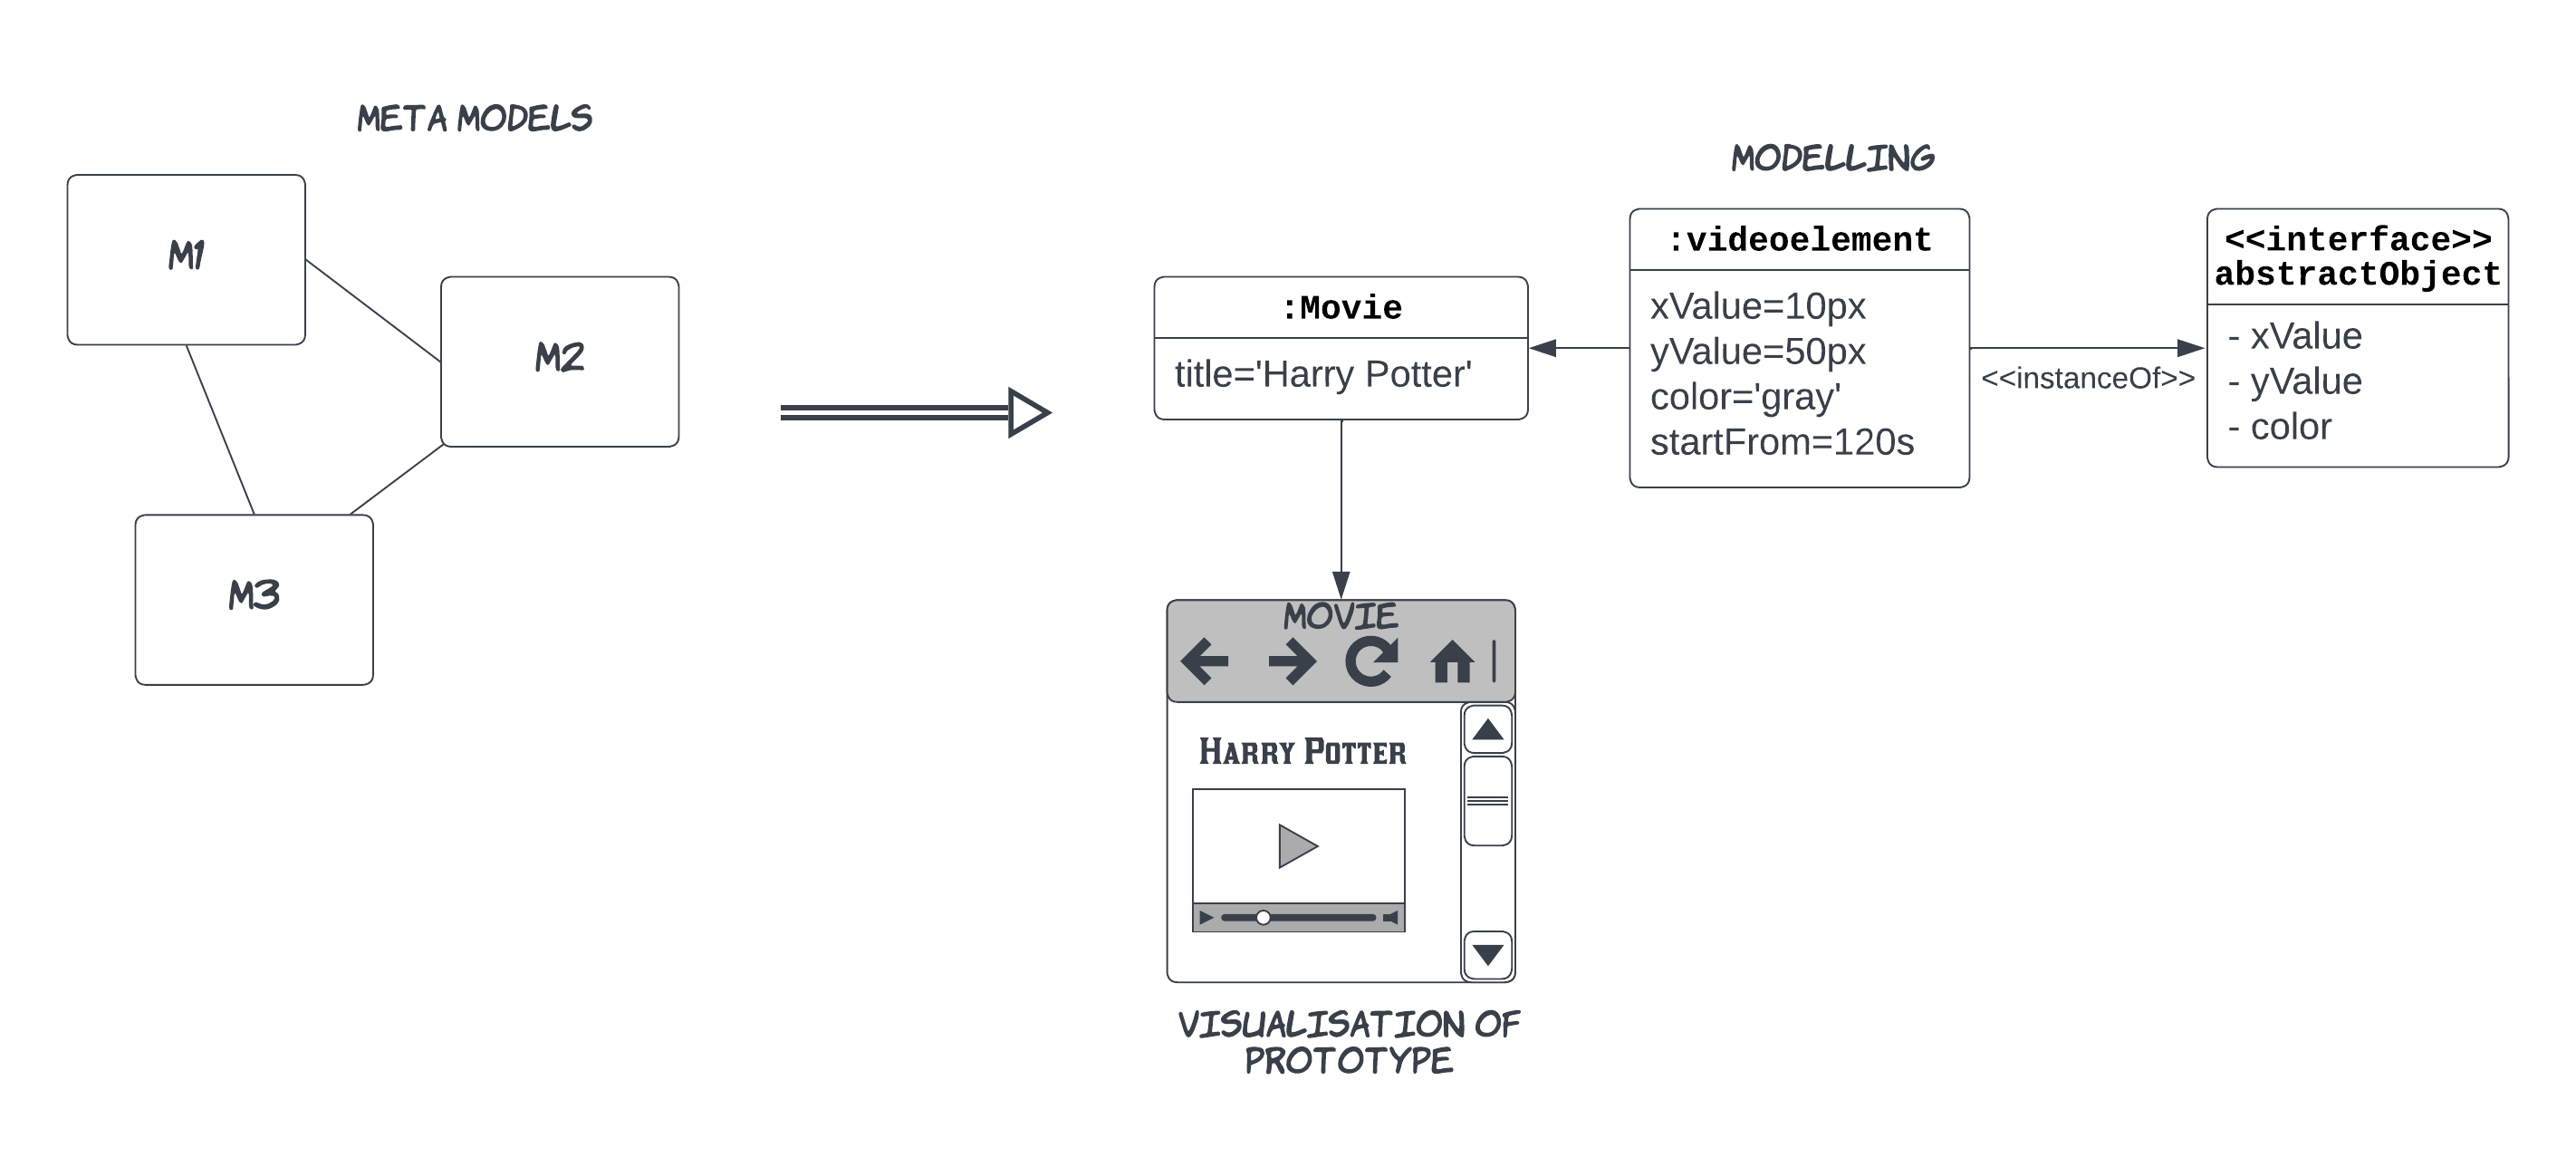
\includegraphics[width=1.05\textwidth]{images/solution-ideas/MetaModel.png}
	\caption{Example Modelling of Prototypes}
	\label{solutionideas:fig:metamodel}
\end{figure}

\paragraph{Prototype:} In the \texttt{Prototype Model}, we store information about the prototypes and all their components as independent parts.
This model stores all the different screens available in a software application and links them.
As per figure \ref{solutionideas:fig:metamodel}, the Modelling part shows the abstract and the concrete models required for prototyping the UI elements. 
(e.g., The ``abstractObject'' is an interface that is inherited by all the UI elements that are concrete elements ``videoelement'' of the containers or the screens ``Movie'').

\paragraph{Experiment:} In the \texttt{Experiment Model}, we store different properties of the UI elements along with the variant information. 
As per figure \ref{solutionideas:fig:metamodel} the ``videoelement'' under modeling contains attributes to store the position of the video viewer, which is a concrete element.
Similarly, it can store some extra properties of the ``videoelement'' that are different from the ``abstractObject''.
Moreover, the models should be able to accept measurements (e.g., \texttt{ClickRate} to measure the user clicks, \texttt{ViewTime} to measure the time spent by the user) to determine the best fit among the variants.
This way, we can create simple Experiments on the users (e.g., changing the position of the UI elements using the drag-and-drop feature).

\paragraph{Task:} In the \texttt{Task Model}, we store a sequence of activities that the user needs to perform and obtain feedback as measurements from the users for testing the software product.
This activity sequence is stored in the models and linked to the users.
The models should be able to accept the Measurements (like the Experiment models) to get feedback from the users (e.g., \texttt{ClickRate} and \texttt{ViewTime}). 

\begin{figure}[h]
	\centering
  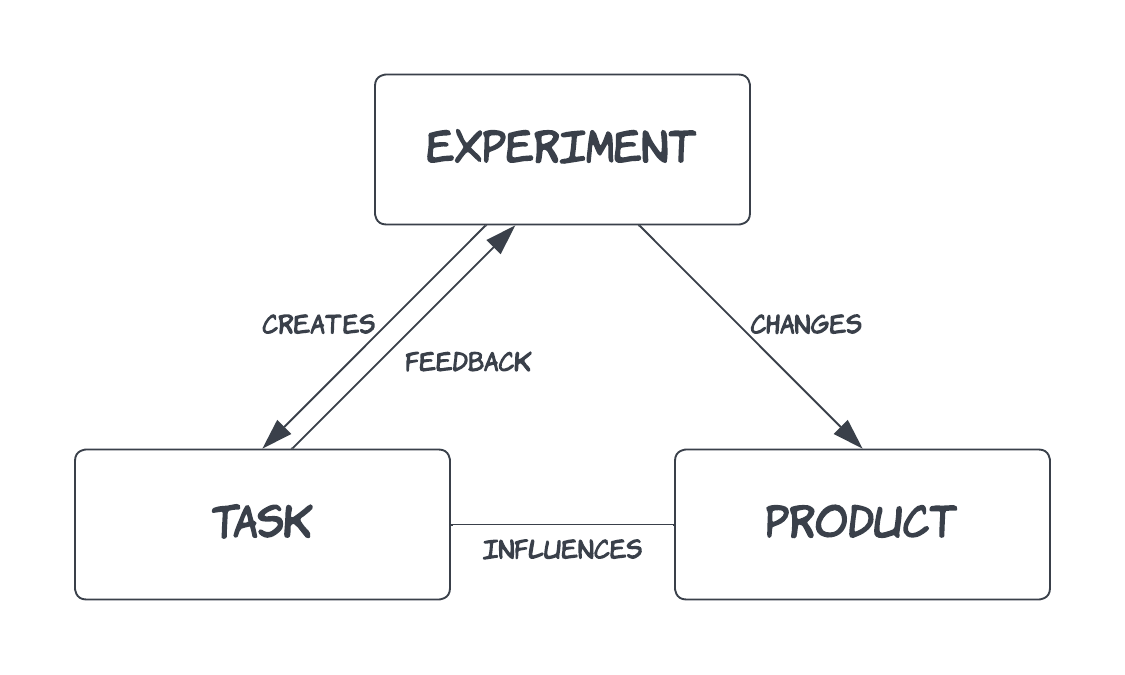
\includegraphics[width=0.7\textwidth]{images/solution-ideas/Triangle.png}
	\caption{Triangle of Experiment, Task, and Prototype}
	\label{solutionideas:fig:triangle}
\end{figure}
% E.g., from \texttt{Videostreamer app}: If the experiment is on a \texttt{Button} element, our model should have information about the position of the button, the style of the button (storing the color, font, etc.), the title of the button, etc. 
% All this information would be stored in the model as its properties or attributes.
% The Model also stores information of different variants of a particular application screen. (E.g., see figure \ref{solutionideas:fig:experimentingvariants} the Grid and the List View)
% E.g., from \texttt{Videostreamer app}: We would give a task to a user U1, saying ``Navigate to the movie M1'' and measure the number of steps/clicks and the time required for the user to perform this task.

We try to relate these models as depicted by the figure \ref{solutionideas:fig:triangle} in a triangle relationship.\\ 
\texttt{(1) Experiment-Task, (2) Experiment-Prototype, and (3) Task-Prototype} relationships.

\paragraph{Experiment-Task:} An experiment can create various tasks for the users and get some feedback in the form of data from the Task model. 

\paragraph{Experiment-Prototype:} From an experiment, it can be decided which is the best variant for the prototype and can thus modify and improve the prototype in an iteratively continuous process.

\paragraph{Task-Prototype:} A task should be created based on the current state of the product, and thus it creates a relationship between the task and the product.


\section{Measure}
The prototypes, experiments, and tasks are ready to be assigned to the users. 
So, in this section, we explain how they are allocated to the users (see section \ref{solutionideas:subsection:usertesting}) and collect feedback (see section \ref{solutionideas:subsection:measurements}) from them for improving the prototypes.

\subsection{Prototypes for User Testing}
\label{solutionideas:subsection:usertesting}

The product owners continuously investigate new features and product enhancement opportunities. 
The owners better understand their customers' experiences by creating that feedback loop with users. 
As a result, they need to conduct experiments.
In these experiments, the population (i.e., all users) is divided into small user groups, each receiving a unique variant. 
This type of setup is called the ``\texttt{Between-group}'' design experiment. 
As mentioned earlier, we also create tasks for the users allocating the tasks to the users performing experiments.  
As shown in figure \ref{solutionideas:fig:experimentingvariants}, the experiment model creates different variants for the prototype \texttt{View}: the \texttt{Grid view} (on the left) and the \texttt{List view} (on the right). 
These experiments are conducted on the users by dividing the users into groups and assigning one of the variants to a group. 
Then, the tasks are created for the specific experiment (e.g., Locate Movie M1). So, all the users with their experiment variant will try to complete the task.
The data are measured (explained in section \ref{solutionideas:subsection:measurements}), analysed (explained in section \ref{solutionideas:section:dataanalysis}), and finally, we find the best variant for the prototype.

\begin{figure}[ht]
	\centering
  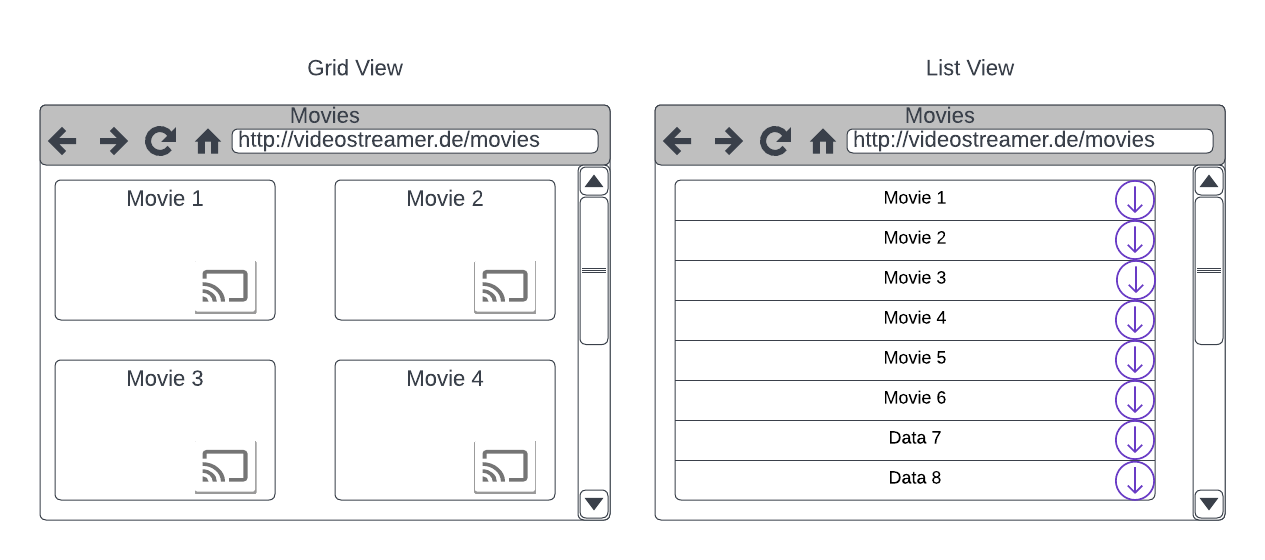
\includegraphics[width=1.0\textwidth]{images/solution-ideas/Experimentvariants.png}
	\caption{Example Experiment variants}
	\label{solutionideas:fig:experimentingvariants}
\end{figure}

\subsection{Measuring the Experiment and Task results}
\label{solutionideas:subsection:measurements}
To measure the experiment variants' performance, we add attributes to the models called ``Measurements''.
This attribute stores the voluntary (e.g., the number of clicks the user makes) and involuntary (e.g., the time required for the user to complete a task) user activities.
This attribute gets updated when the users perform the Task assigned to them by the \texttt{Task Model}.
(e.g., The task is to locate a movie for a registered user, so the user must log in, go to the movies page and search for the film, or scroll to find the film and click on the movie's title to play it.)
The UI variant (List or Grid View) assigned to the user plays a vital role in making this process smooth.
Therefore, measuring the Time or the Clicks required to reach the goal can be a critical factor in deciding the better variant.
After collecting the data from the experiment variants, we do an analyses (see section \ref{solutionideas:section:dataanalysis}) and improve prototype (see section \ref{solutionideas:subsection:improvingprototypes})

\section{Learn}
In this section, we do the analyses (see section \ref{solutionideas:section:dataanalysis}) from the data collected during the Experiments, get feedback on the better experiment's variant, and improve our prototype (see section \ref{solutionideas:subsection:improvingprototypes}).
\subsection{Analysis}
\label{solutionideas:section:dataanalysis}

In our solution, we focus on data-driven development. 
To determine the ``Winner'' among the variants of a product's component, we perform data analytics on the feedback data we receive from the \texttt{Task Model} and the \texttt{Experiment Model}.
We perform the \texttt{Quantitative} (presented in section \ref{solutionideas:paragraph:quantitative}), \texttt{Qualitative} (presented in section \ref{solutionideas:paragraph:qualitative}), and the \texttt{Task} (presented in section \ref{solutionideas:paragraph:taskanalysis}) analyses of the data.

% \begin{figure}[ht]
% 	\centering
%   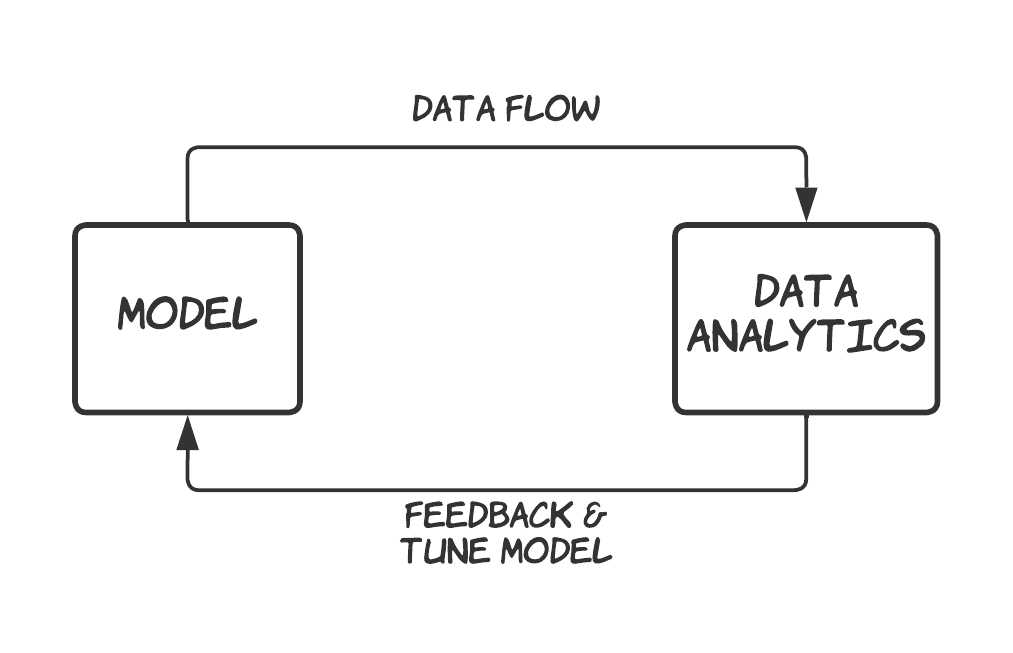
\includegraphics[width=0.5\textwidth]{images/solution-ideas/dd-development.png}
% 	\caption{Model-based \& Data Driven development}
% 	\label{solutionideas:fig:dddevelopment}
% \end{figure}

\paragraph{Quantitative Analysis:}
\label{solutionideas:paragraph:quantitative}
Quantitative analysis uses mathematical and statistical methods to determine the behavior of the data.
In quantitative research, various descriptive statistics methods like Means, Median, Variances, Standard Deviations, etc., are used to find some causal relationships in the data.
After collecting the data, the experimenting server can calculate the measurements' mean (assume the mean is specified in the experiment).
But, it isn't easy to generalize the results using means or descriptive statistical methods. 
Therefore, a significance test can be calculated to validate the probability of the event's occurrence, claim from the mean, and declare the winner variant.

\paragraph{Qualitative Analysis:}
\label{solutionideas:paragraph:qualitative}
To further improve, we need to perform qualitative analysis.
Qualitative analysis is used to determine the users' behavior and semantics.
Qualitative research data is usually unstructured, coming from open-ended surveys, interviews, etc. 
Our goal is to turn the unstructured data into a detailed description of the critical aspects of the problem.
In our solution, we propose to perform a qualitative analysis of the data by asking some open-ended questions to the users
(e.g., questions like ``What do you think about the Look and feel of the software application?'', ``Are the items on the page easily locatable?'', etc.).
The users' responses can be studied using some tools using the inductive or deductive coding technique. 
% If we select the inductive coding approach, we will scrutinize the reactions and those which are similar and group them. 
% These groups will be coded into labels, and we will formalize and analyze the categories. 
% To understand the process better, see figure \ref{solutionideas:fig:qualitative}. 
So, in the end, we get feedback from this process on which variants are better for the users. 
This information is forwarded to the models for modifying the prototypes.

% \begin{figure}[ht]
% 	\centering
%   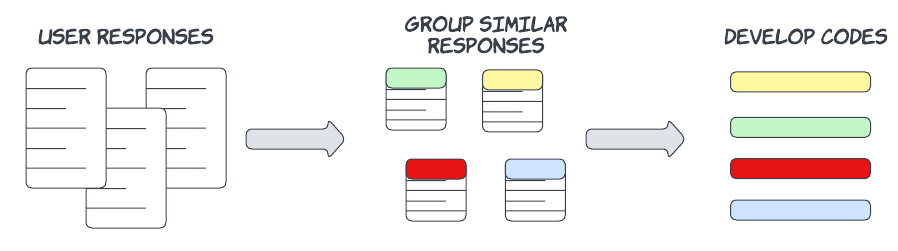
\includegraphics[width=1\textwidth]{images/solution-ideas/qualitative.png}
% 	\caption{Qualitative analysis using inductive coding}
% 	\label{solutionideas:fig:qualitative}
% \end{figure}

\paragraph{Task analysis:}
\label{solutionideas:paragraph:taskanalysis}
We also receive the data from the \texttt{Task Model}. 
Its data can be used to calculate the efficiency of the variant. 
A task model contains measurements for getting feedback from the users. 
E.g., If the task is to locate a particular movie, we can calculate the number of clicks and time required as measurements for the users to reach their destination.
This testing type is called ``\texttt{Supervised testing}'' \cite{article:dataanalysis:supervisedtest}.
So, we observe the users, and they know the result (i.e., the movie they need to locate). 
This process gives us more accurate feedback on which variant performs better, and we can then update the prototype as per our triangle relationship (see fig \ref{solutionideas:fig:triangle}).

\subsection{Improving the Prototype}
\label{solutionideas:subsection:improvingprototypes}
As per the LEAN development process, this is the final step in the cycle (see figure \ref{intro:fig:lean}) of that iteration.
After analyzing the data from experiments, we can conclusively claim with statistical evidence the ``winner'' variant of a component.
This helps us to tune our model by adding a ``default'' attribute and setting its value to be of the ``winner'' variant.
So, in the next iteration cycle, for the component, the ``winner'' variant is selected as default for future experiments.
After modifying our model, we can visualize the changes by observing the UI Prototypes.
E.g., In the \texttt{View} component of the \texttt{Videostreamer} app, the \texttt{GridView} is determined to be more usable as per the experiment and is declared the winner. 
Therefore, in the next iteration, the \texttt{default} attribute in the \texttt{View} component will be set to \texttt{GridView} for the following experiments.